\section{Submission}
\label{sec:results}

Next, we describe the tools and the data we exploited for feature extraction, the data used to train the classifier, and the results of our participation in the shared task.

\subsection{Feature Extraction}

We need to generate two types of models to extract our features: probabilistic lexicons and language models. We used the probabilistic lexicons that can be obtained as a sub product of the training of full statistical models. In particular, we used Moses~\cite{Moses} with its default configuration with the News Commentary V13 parallel corpus as provided for the News translation shared task. We used the same corpora to train the language models. For this, we used Kenlm~\cite{Kenlm} and estimated models of order $5$.


\subsection{Training the classifier}
\label{ssec:data}

We also used News Commentary V13 parallel corpus for training the classifier. We generated as many negative examples as positive sentence pairs in the corpus for a total of almost $600$k data points. The negative examples were evenly distributed among the thee perturbation operations described in the previous section. We used the implementation of gradient boosting classifier from the scikit-learn library\footnote{\url{http://scikit-learn.org/stable/index.html}} to train our model. The model was then applied to each sentence pair in the noisy Paracrawl corpus from the shared task. We used the probability of the positive class as predicted by the classifier as the final scores in our submission.

We also conducted some initial experiments using the Common Crawl corpus, under the rationale that it would be closer to the domain of the noisy data from the Paracrawl corpus. However, Common Crawl data has quite a large number of misaligned sentences. To handle this issue we implemented an iterative training process which comprises the following steps: a) train the model using all available data as positive class and synthetically generated data as negative class (see Sec); b) use the trained model to clean the available data eliminating the sentence pairs assigned to the negative class with a very high probability; c) use the cleaned data to train a new model; d) repeat until no more sentence pairs can be eliminated with a given threshold. An advantage of this approach is that it allows to be less dependent on the quality of the initial training data. However, we had to stop exploring this direction due to time constraints.


%https://docs.google.com/spreadsheets/d/1SKMOBbH5YVsQJpbUCMN3K8Gzt_89zBabQl716Aw8NjM/edit?usp=sharing
\begin{figure}[ht]
  \centering
  \begin{subfigure}[b]{\columnwidth}
    \hspace*{-1.5em}
    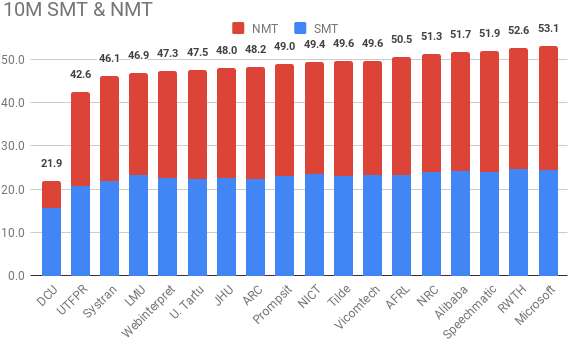
\includegraphics[width=1.1\textwidth]{images/10M_crop.png}
    \label{fig:10M}
  \end{subfigure}
  ~
  \begin{subfigure}[b]{\columnwidth}
    \hspace*{-1.5em}
    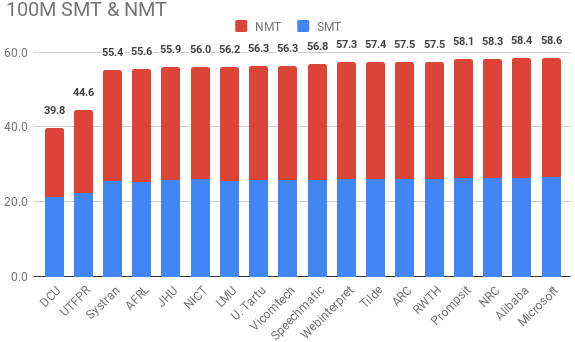
\includegraphics[width=1.1\textwidth]{images/100M_crop.png}
    \label{fig:100M}
  \end{subfigure}
  \caption{Best submission of each participant institution. We display BLEU [\%] results stacked for SMT (\textcolor{blue}{blue}) and NMT (\textcolor{red}{red}).}
  \label{fig:results}
\end{figure}

\subsection{Evaluation and results}

Participants in the shared task have to submit a file with quality scores, one per line, corresponding to the sentence pairs on the 1 billion word German–-English Paracrawl corpus. Scores do not have to be meaningful, except that higher scores indicate better quality. The performance of the submissions is evaluated by sub-sampling $10$ million and $100$ million word corpora based on these scores, training statistical~\cite{Moses} and neural~\cite{Marian} MT systems with these corpora, and assessing translation quality on six blind test sets\footnote{Tests: newstest 2018, iwslt 2017, Acquis, EMEA, Global Voices, and KDE.} using the BLEU~\cite{Bleu} score. 

Figure~\ref{fig:results} displays the score of the best submission of each individual participant institution. The top plot shows the results for the $10$ million token sub-sampled corpus, and the bottom plot shows the results for the $100$ million token corpus. Scores are the aggregation of the BLEU scores of the statistical and neural systems averaged over the six blind test sets.

One first observation we can make is that (almost) all scores are quite close to each other with little variation between them; particularly in the $100$ million condition. Also, the scores for the statistical and neural systems tend to follow the same pattern. We do not have confidence intervals available which makes difficult to interpret the observed differences between systems. Still, in the case of $100$ million tokens sub-sampling, it seems quite clear that all the systems except for the DCU and UTFPR submissions are of the same quality. There is only a $5\%$ relative improvement between the last system of this group and the best submission to the task. Scores are a bit more spread out in the $10$ million tokens sub-sampling. This indicates that $100$ million sample neutralizes the differences between the data cleaning methods and allows (almost) all systems to reach a theoretical maximum.

Our submission (Webinterpret) scored $22.5$ for statistical and $24.8$ for neural MT systems on the $10$ million tokens sub-sampling, in comparison to the corresponding scores of $24.5$ and $28.6$ achieved by the best submission. For the $100$ million condition, we scored $26.1$ and $31.2$, in comparison to the best system with the respective scores of $26.5$ and $32.1$. 
